\graphicspath{{02-TOF/Figures/}}


\newcommand{\mchange}[2]{{\color{red}#1}{\color{green}#2}}
\newcommand{\malert}[1]{{\it\color{red}#1}}


\section{Time-of-Flight Detectors}
\label{Sect:TOF}

List of figures
\begin{itemize}
\item PMT charge correlation PMT0 vs PMT1 - maybe, if relevant
\item TW calibration of one channel
\item Slab DT before TW correction and after - single pixel.
\item Residual TW
\item T0 correction for 1 channel - electron peak fit
\item Slab DT mean and sigma for all pixels after calibration
\item Overall slab DT
\item Space-point creation efficiency per pixel/slab
\item Particle detection efficiency - don't know how to extract from
  the data, ideally pixel map for each TOF
\end{itemize}


\subsection{Introduction}
\label{SubSect:TOF_Intro}
% version 01 edited by Maurizio Bonesini 19/2/2018

Three time-of-flight detectors (TOF0, TOF1, TOF2) have been built and installed at RAL in 2008 and 2009 to measure the position and the time of crossing particles.
TOF0 and TOF1~\cite{NOTE145},~\cite{NOTE241},~\cite{2010NIMPA.615...14B} are placed upstream of the cooling channel, and TOF2~\cite{NOTE286} is downstream of the channel, mounted in front of the KL, as shown in~Fig.~\ref{fig:BL}.
The time of flight between two TOF stations provides particle identification information and can also be used for momentum measurement. TOF1 served most of the time also as an experimental trigger.
They  have smoothly operated during the so-called Step~I and Step~IV~\cite{Rajaram:2015bra},~\cite{2015ehep.confE.521B} running periods of the MICE experiment and were essential for all the measurements done.

The good performances of the TOF detectors, over an extended period of time,
has enabled the MICE experiment to characterize fully its muon beams during
Step~I data-taking, by measuring their emittance~\cite{2013arXiv1306.1509T} and
assessing their pion contamination~\cite{2016JInst..11P3001A}.

Each TOF station is made of two planes of fast~1" thick scintillator counters
along X/Y directions (to increase measurement redundancy) read out at both edges by
R4998 Hamamatsu fast photomultiplier tubes\footnote{one-inch linear
focused PMTs with 10 stages, typical gain G$\sim$5.7$\times$10$^6$
at -2250~V and B=0~T, rise time 0.7~ns, transit time spread (TTS)~$\sim$160~ps}.
R4998 PMTs have been delivered by Hamamatsu in assemblies (H6533MOD) that
include the PMT tube, the voltage divider chain and a 1~mm thick $\mu$-metal
shield, extending 30~mm beyond the photocathode surface.
\mchange{The}{To} increase the count rate stability active dividers were used, instead of
conventional resistive ones.
A simple design with flat fish-tail PMMA light guides, as \mchange{respect}{opposed} to tilted ones
(to reduce the influence of magnetic field) or Winston cones, has
been chosen to optimize the timing detector resolution (favouring
the collection of straight light) and to allow an easy mechanical
assembly. \malert{any picture or reference here?}
TOF0, TOF1, and TOF2 have active areas of 40$\times$40~cm$^2$, 42$\times$42~cm$^2$, and 60$\times$60~cm$^2$ respectively.
The slabs in TOF0 are 4~cm wide, while the slabs of TOF1 and TOF2 are 6~cm wide respectively.
The PMT\mchange{s}{} signal, after $\sim$34~m long RG213 cable and a $50\%-50\%$ passive
splitter, arrive to a leading-edge CAMAC Lecroy 4115 discriminator
followed by a CAEN V1290 TDC for time measurements and to a CAEN V1724 FADC
for pulse-height measurements, to correct time-walk. As reported in
reference~\cite{NOTE241}, RG213 cables\footnote{CERN type C-50-6-1, with
rated delay 4.08 ns/m} have a better temperature stability
than conventional RG58 cables. Their delay have been individually measured
in laboratory, before installation in the experimental hall.
Time calibration of individual counters has been done with impinging beam particles by using the detector
X/Y redundancy~\cite{NOTE251}. \malert{This is too vague. Calibration
  will be covered later. What does counter refer to here?}

Due to the low residual magnetic field produced by the last quadrupole
of the beam line in the proximity of the TOF0 detector ($\leq$50~G),
the used conventional PMTs had to use  elongated $\mu$-metal
shielding.
The other two TOF stations (TOF1/TOF2) had to work instead in the stray fields
of the cooling channel solenoids, that are only partially shielded by a 100~mm thick
annular iron plates. As residual magnetic fields are up to 0.13~T (with a
component along the PMTs axis up to 0.04~T), a local or global
magnetic shielding for TOF1 and TOF2 detectors had to be envisaged.
The local shielding option was chosen, at the end, for convenience and
easiness of implementation.
As magnetic shielding is a mass effect, box-shaped soft iron shielding
are more effective than cylindrical ones. This idea pioneered in the
D0 experiment has been tested in the case of MICE using different geometrical
configuration for the iron shielding boxes and different iron materials (e.g. Fe360, ARMCO\footnote{ARMCO steel from AkSteel is a pure iron with
a maximal carbon content of $0.025\%$ and very high magnetic saturation},~etc).
The problem is usually the longitudinal component of the magnetic field, while the orthogonal component may be more easily shielded.
Systematic studies have been done, using a built on purpose solenoid of 23~cm inner diameter,
40~cm length\footnote{built by TBM srl, Uboldo (VA), Italy} and are fully reported in reference~\cite{2012NIMPA.693..130B}.
A composite structure based on the 1~mm $\mu$-metal shielding
of the H6533Mod assemblies and an external
additional 6$\times$6~cm$^2$ (5.6$\times$5.6~cm$^2$) ARMCO box, 15~cm long, with an
internal hole of 3.2~cm diameter has been adopted for the PMT's magnetic
shielding of TOF2 (TOF1)~\cite{NOTE455}.
Fig.~\ref{fig:TOF1} show how the local shielding has been
implemented in TOF2, using different sheets of ARMCO to make a ``single bar structure''
for all the PMTs of one side, instead of single boxes for individual PMTs. The effective shielding amounts to $\sim$6.6~cm of ARMCO
thickness, with extra shielding effect due to the fact that all bars shielding
the TOF2 PMTs are magnetically linked between them and to both the KL shielding
and the shielding  plate making a single magnetic loop.
\begin{figure}
  \begin{center}
  \includegraphics[width=9cm,angle=-90]{./02-TOF/Figures/TOF2.eps} \\
  \caption{Exploded view of the TOF2 detector magnetic shielding for one row of PMTs.}
  \label{fig:TOF1}
  \end{center}
\end{figure}
Fig.~\ref{fig:TOF2} shows some steps of the assembly procedure for the TOF2
detector at INFN MIB mechanics workshop.
\begin{figure}
  \begin{center}
  \includegraphics[width=0.24\columnwidth]{./02-TOF/Figures/TOF_assembly_a.png}
  \includegraphics[width=0.24\columnwidth]{./02-TOF/Figures/TOF_assembly_b.png}
  \includegraphics[width=0.24\columnwidth]{./02-TOF/Figures/TOF_assembly_c.png}
  \includegraphics[width=0.24\columnwidth]{./02-TOF/Figures/TOF_assembly_d.png}
  \caption{Assembly of TOF2 at INFN MIB mechanics workshop. Left to right: from the bare magnetic shielding to the installed counters of a plane.}
  \label{fig:TOF2}
  \end{center}
\end{figure}

\malert{The paragraph above is rather detailed, with many things that
  could be explained incorrectly. Should be made brief, unless full
  technical design description is required.}


\malert{The following paragraph is summarising the performance. It
  states overly optimistic performance.}

For what attains performances, TOF0, TOF1, and TOF2 had timing
resolutions around 50-60 ps respectively \malert{(currently observed
  $\sim$110~ps)},
over the 8 years running period, consistent with design requirements,
with the spatial resolution around 1~cm. \malert{We don't use any
  special reconstruction method. Resolution kept at 4 cm or 6 cm for
  TOF0 or TOF1 and TOF2 respectively. Do we say resolution = 1/2 of
  strip width or $1/\sqrt{12}$?}
Fig.~\ref{fig:TOF3}~shows distributions of the time of flight between TOF0 and TOF1 where electrons, muons and pions fall into three well defined peaks.
\begin{figure}
  \begin{center}
    \includegraphics[width=0.6\columnwidth]{./02-TOF/Figures/TOF.png}
    \caption{Time of flight between TOF0 and TOF1 for a ``pion'' beam. From the left: the well separated electron, muon and pion peaks.}
    \label{fig:TOF3}
  \end{center}
\end{figure}


\malert{What is currently the main purpose of TOFs? This determines
  the requirements on the performance. Will need to tell that current
  T-o-F measurement has sufficient resolution, which appears to be
  $\sim$100-120~ps}


\subsection{TEMPORARY - Plots}

\begin{figure}
  \begin{center}
  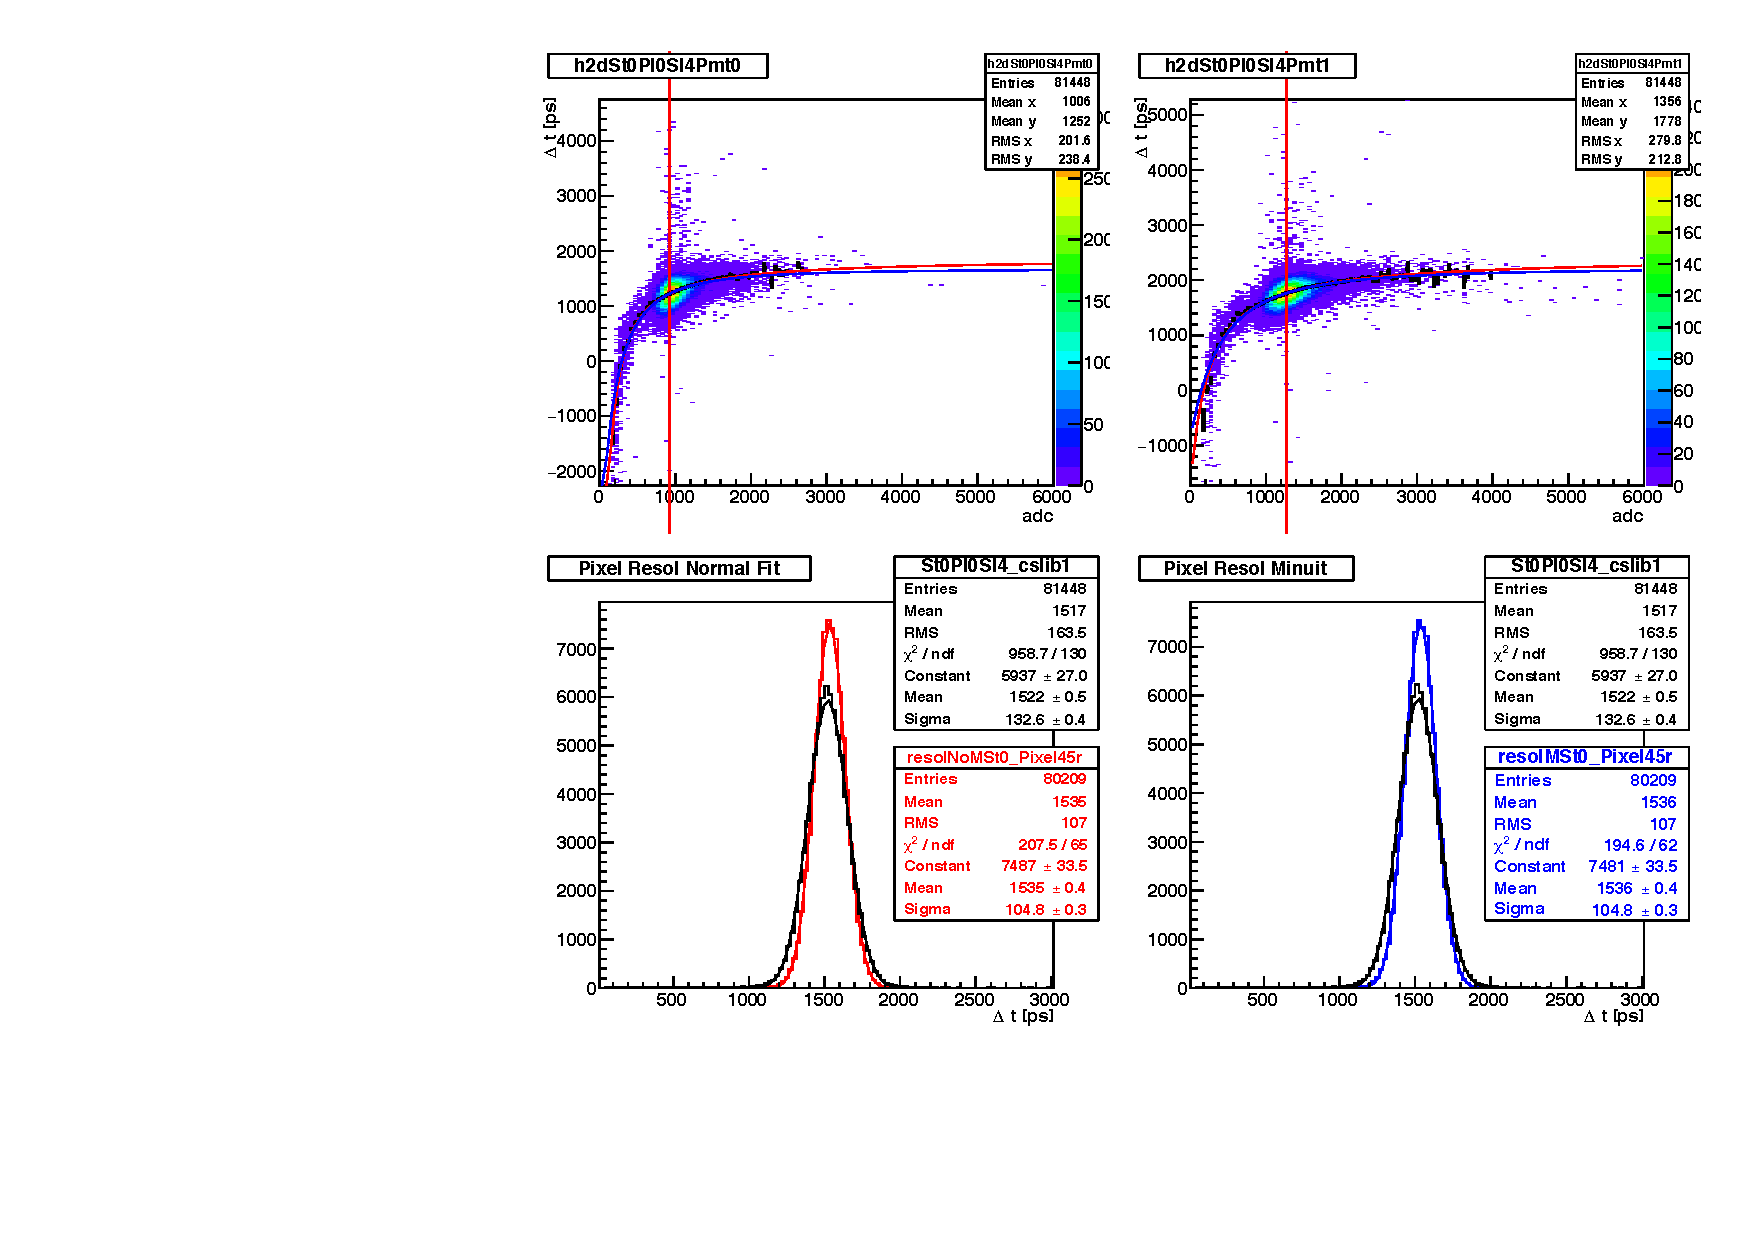
\includegraphics[clip,trim=0 8.5cm 10cm 0, width=9cm]{01_tw_example} \\
  \caption{}
  \label{fig:TW}
  \end{center}
\end{figure}

\begin{figure}
  \begin{center}
  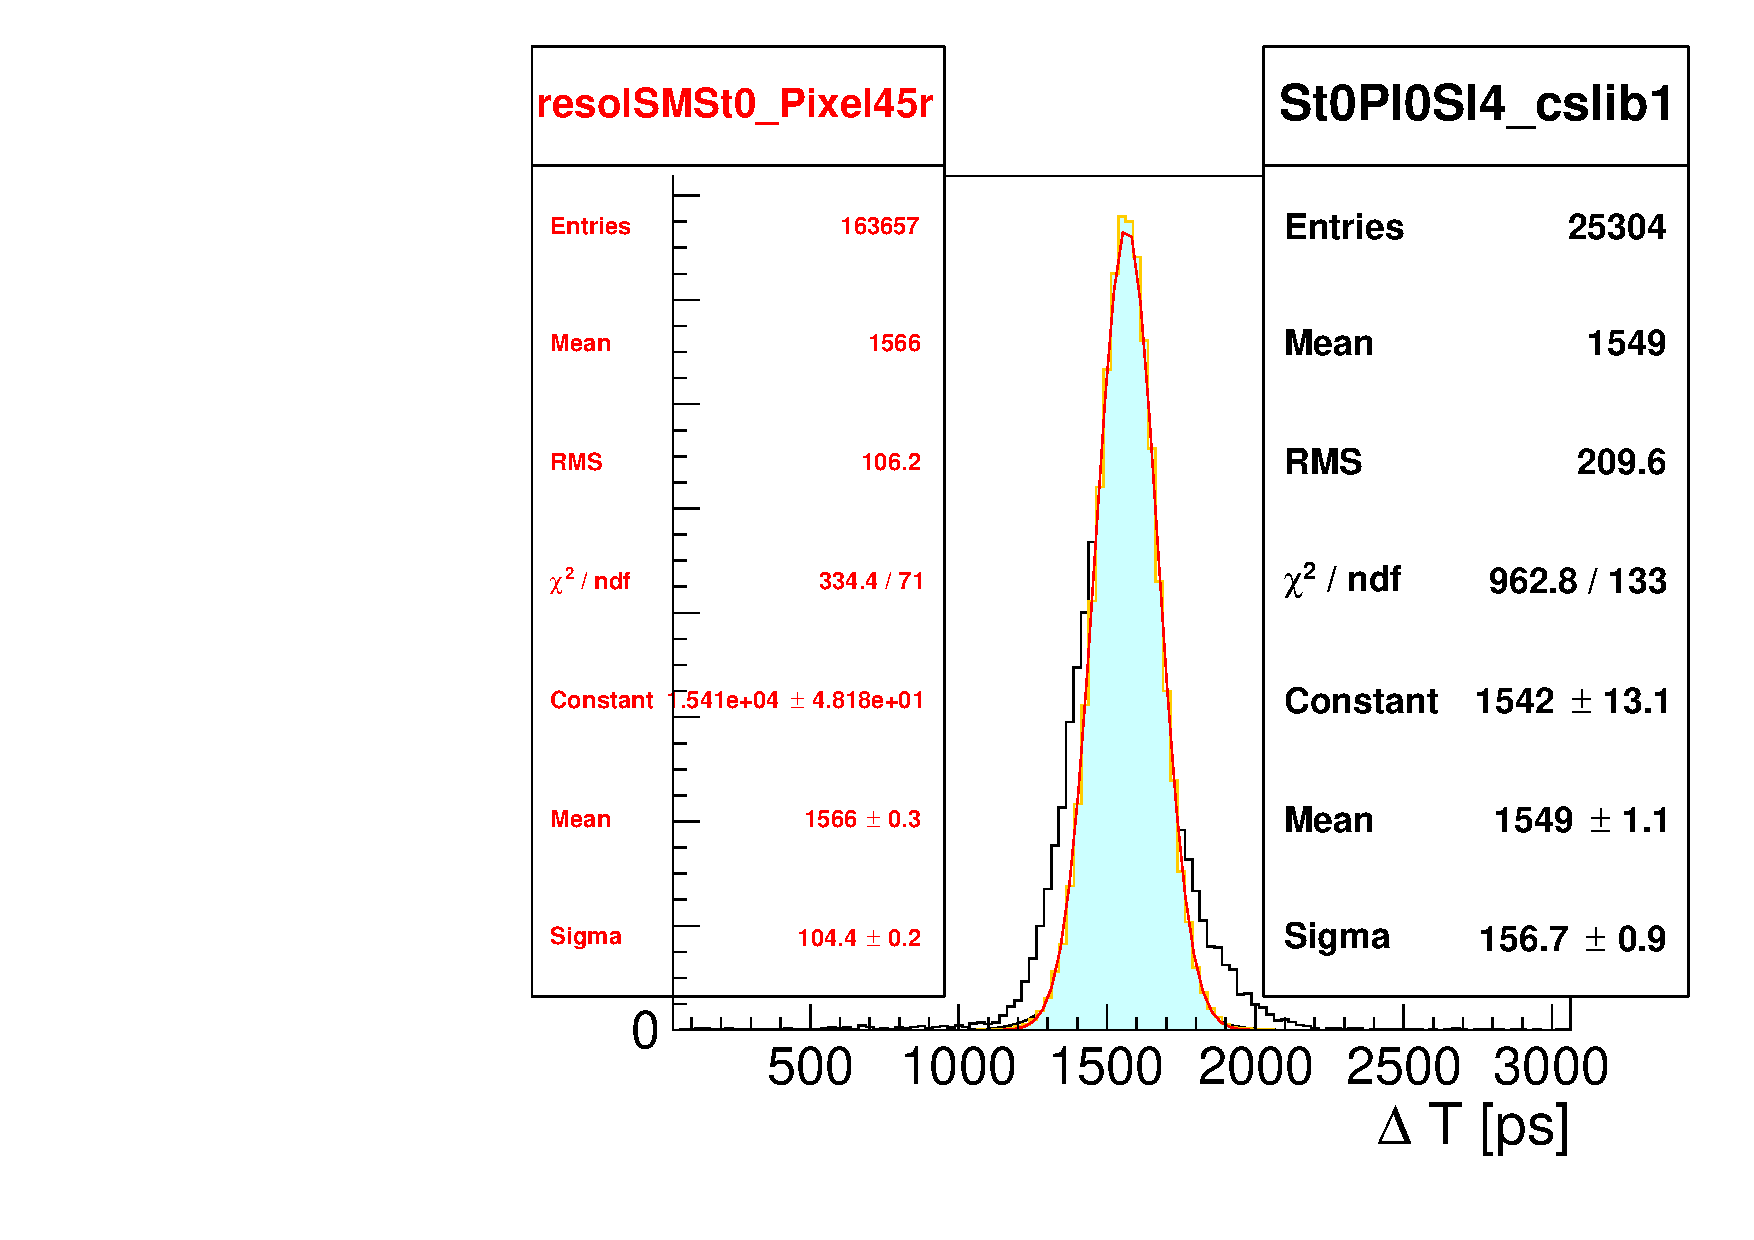
\includegraphics[clip,trim=0 0 10cm 8.5cm, width=9cm]{02_slab_dt_resolution_tw_effect} \\
  \caption{}
  \label{fig:SlabDTTW}
  \end{center}
\end{figure}

\begin{figure}
  \begin{center}
  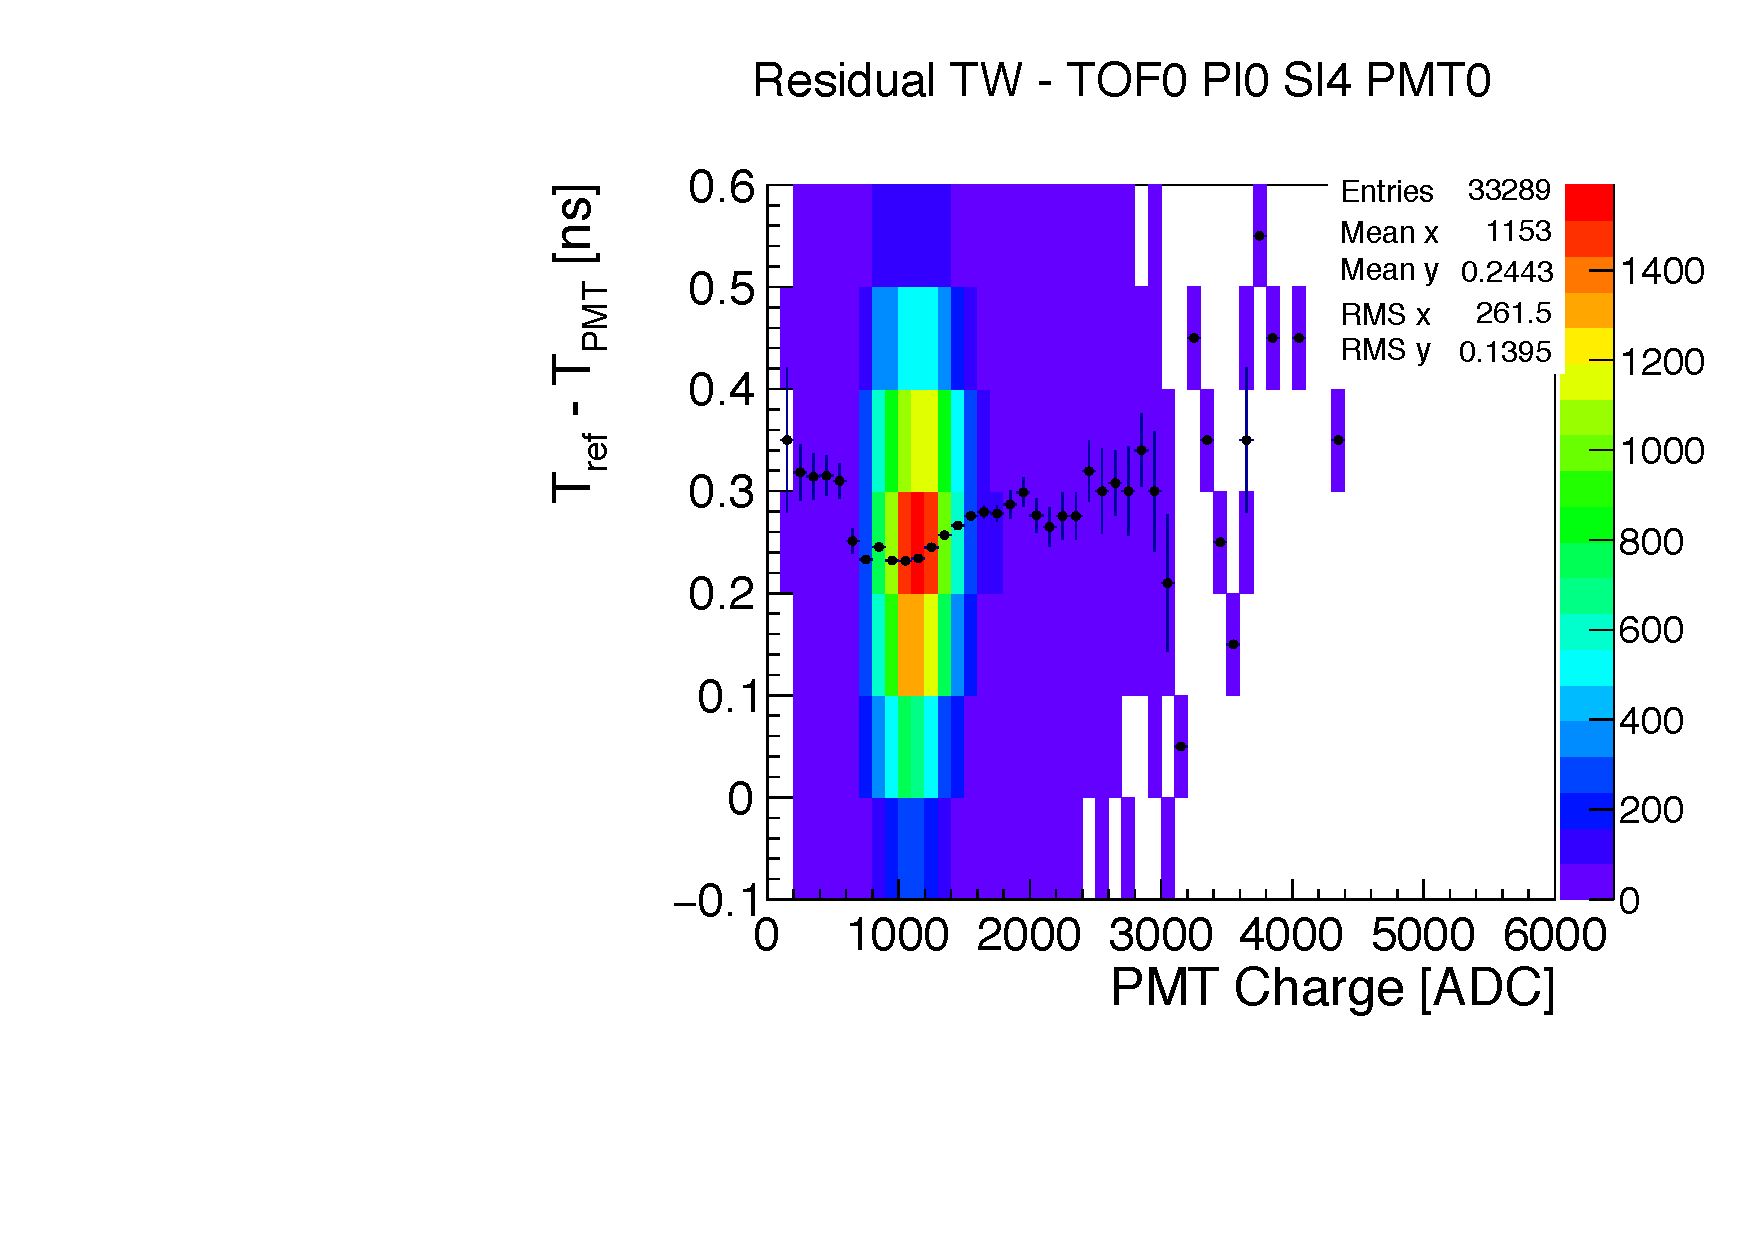
\includegraphics[width=9cm]{03_residual_tw_example} \\
  \caption{}
  \label{fig:ResTW}
  \end{center}
\end{figure}



\begin{figure}
  \begin{center}
  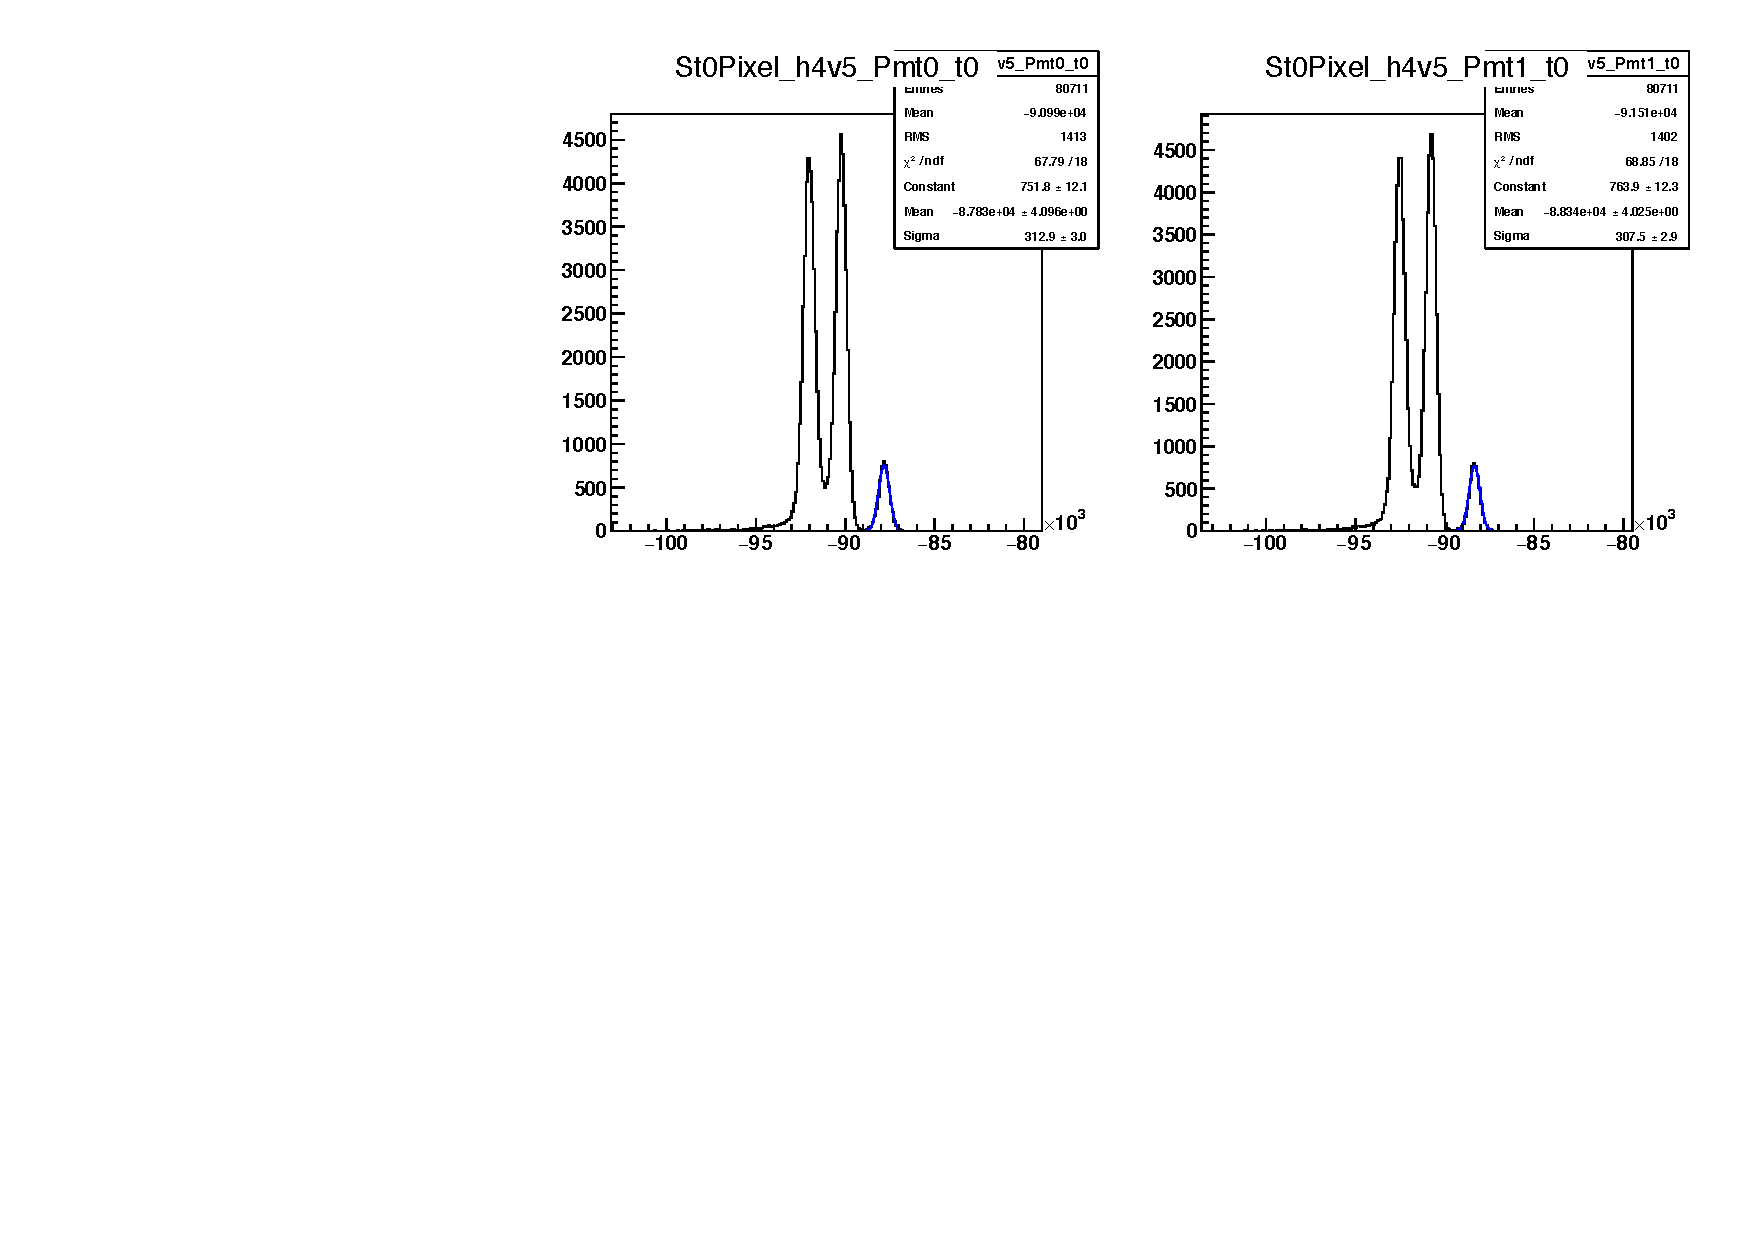
\includegraphics[clip,trim=0 0cm 10cm 0, width=9cm]{04_tof_t0_example} \\
  \caption{}
  \label{fig:tofT0}
  \end{center}
\end{figure}


\begin{figure}
  \begin{center}
  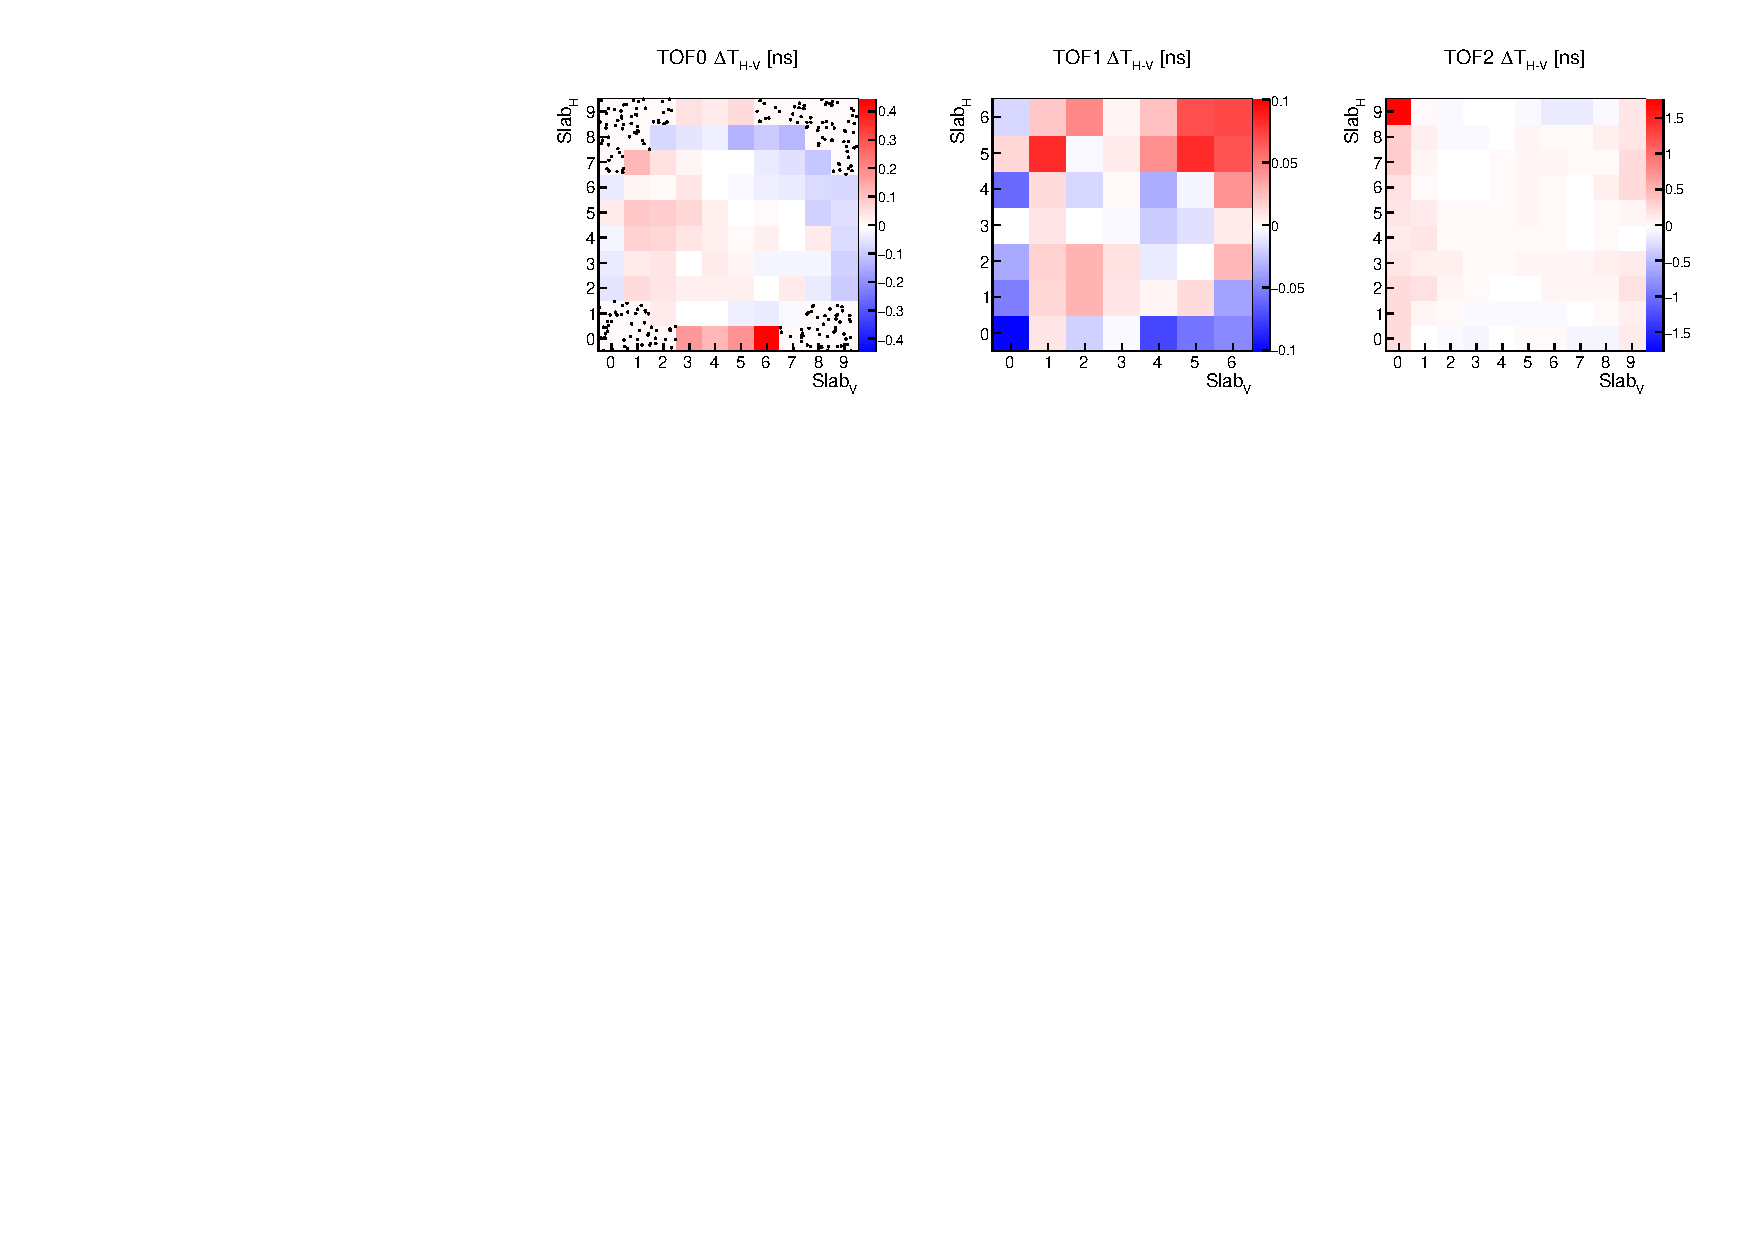
\includegraphics[width=15cm]{05_slab_dt_offset_by_pixel_2d} \\
  \caption{}
  \label{fig:SlabDToffsetByPixel}
  \end{center}
\end{figure}


\begin{figure}
  \begin{center}
  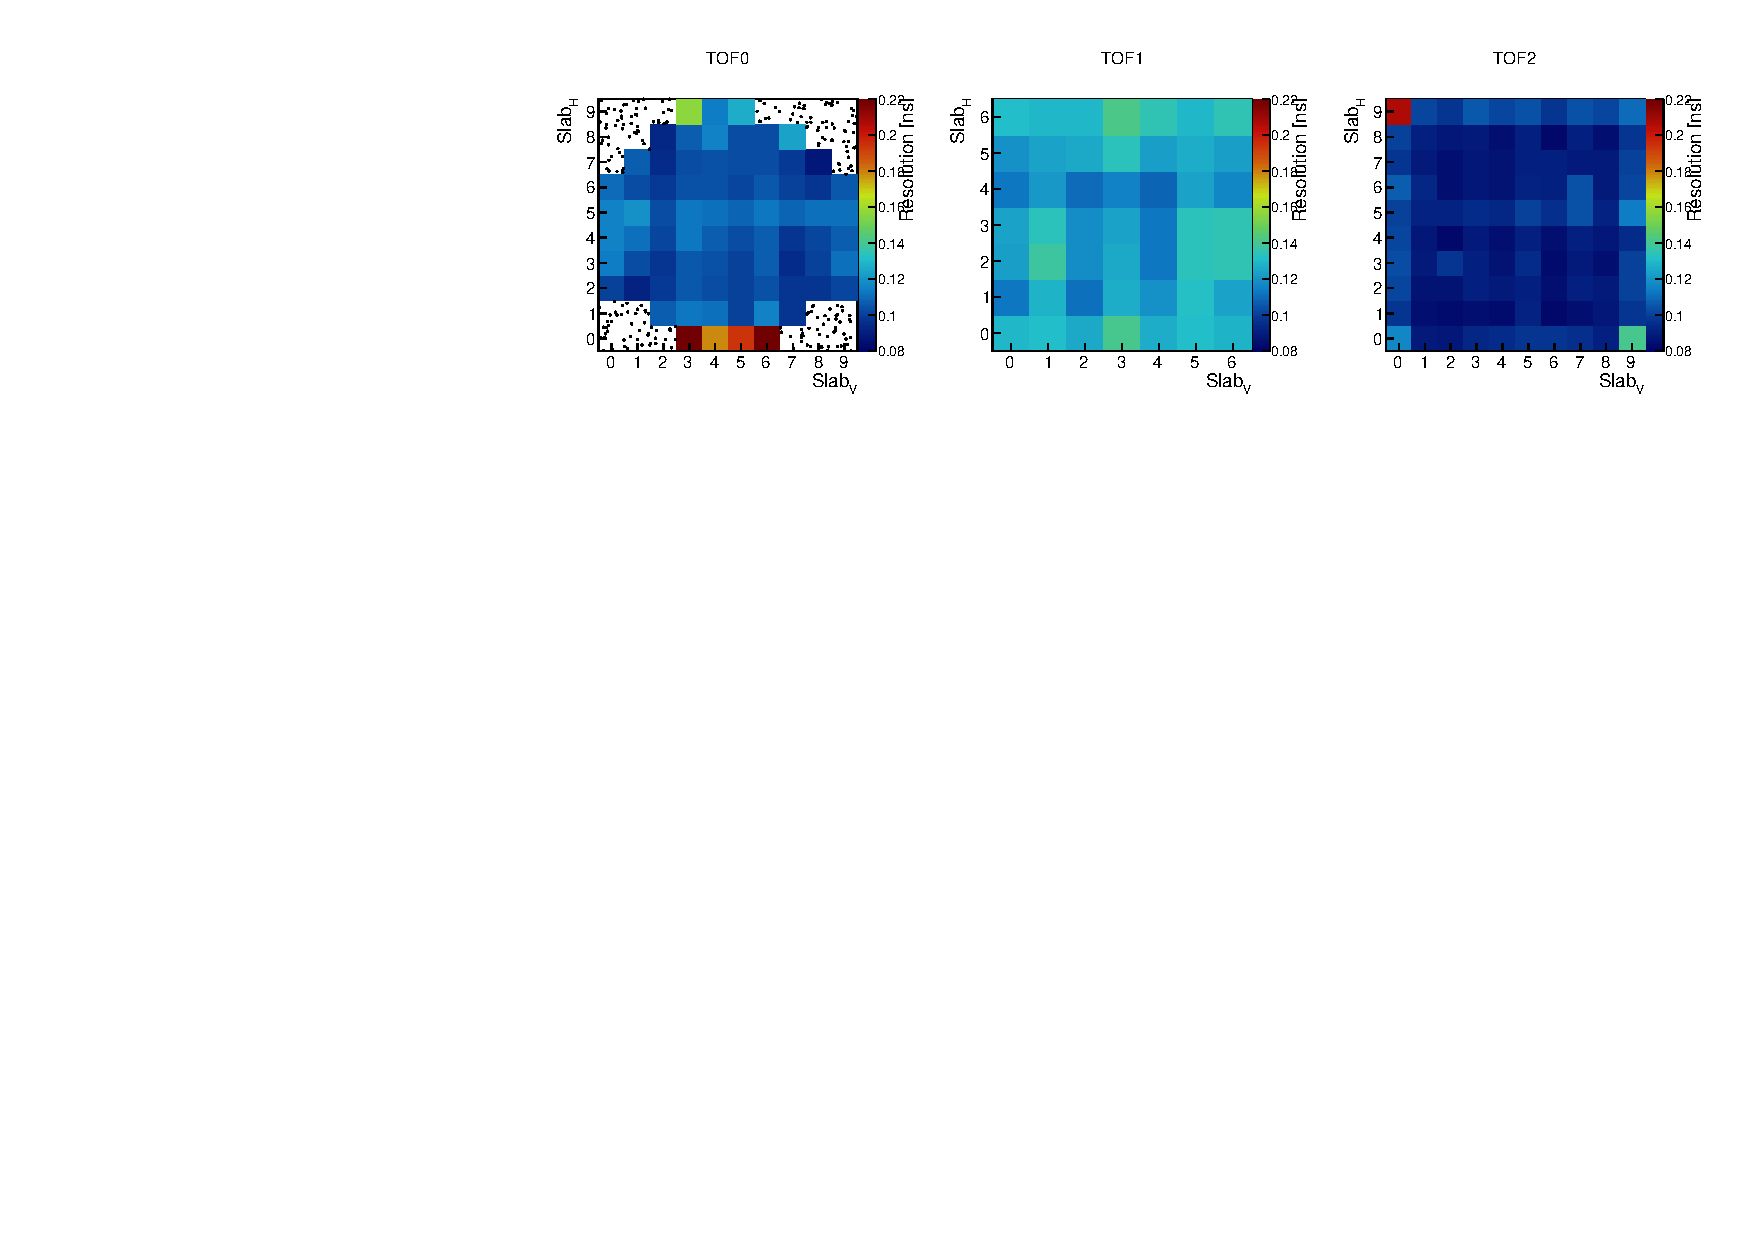
\includegraphics[width=15cm]{06_slab_dt_resolution_by_pixel_2d} \\
  \caption{}
  \label{fig:SlabDTresByPixel}
  \end{center}
\end{figure}



\begin{figure}
  \begin{center}
  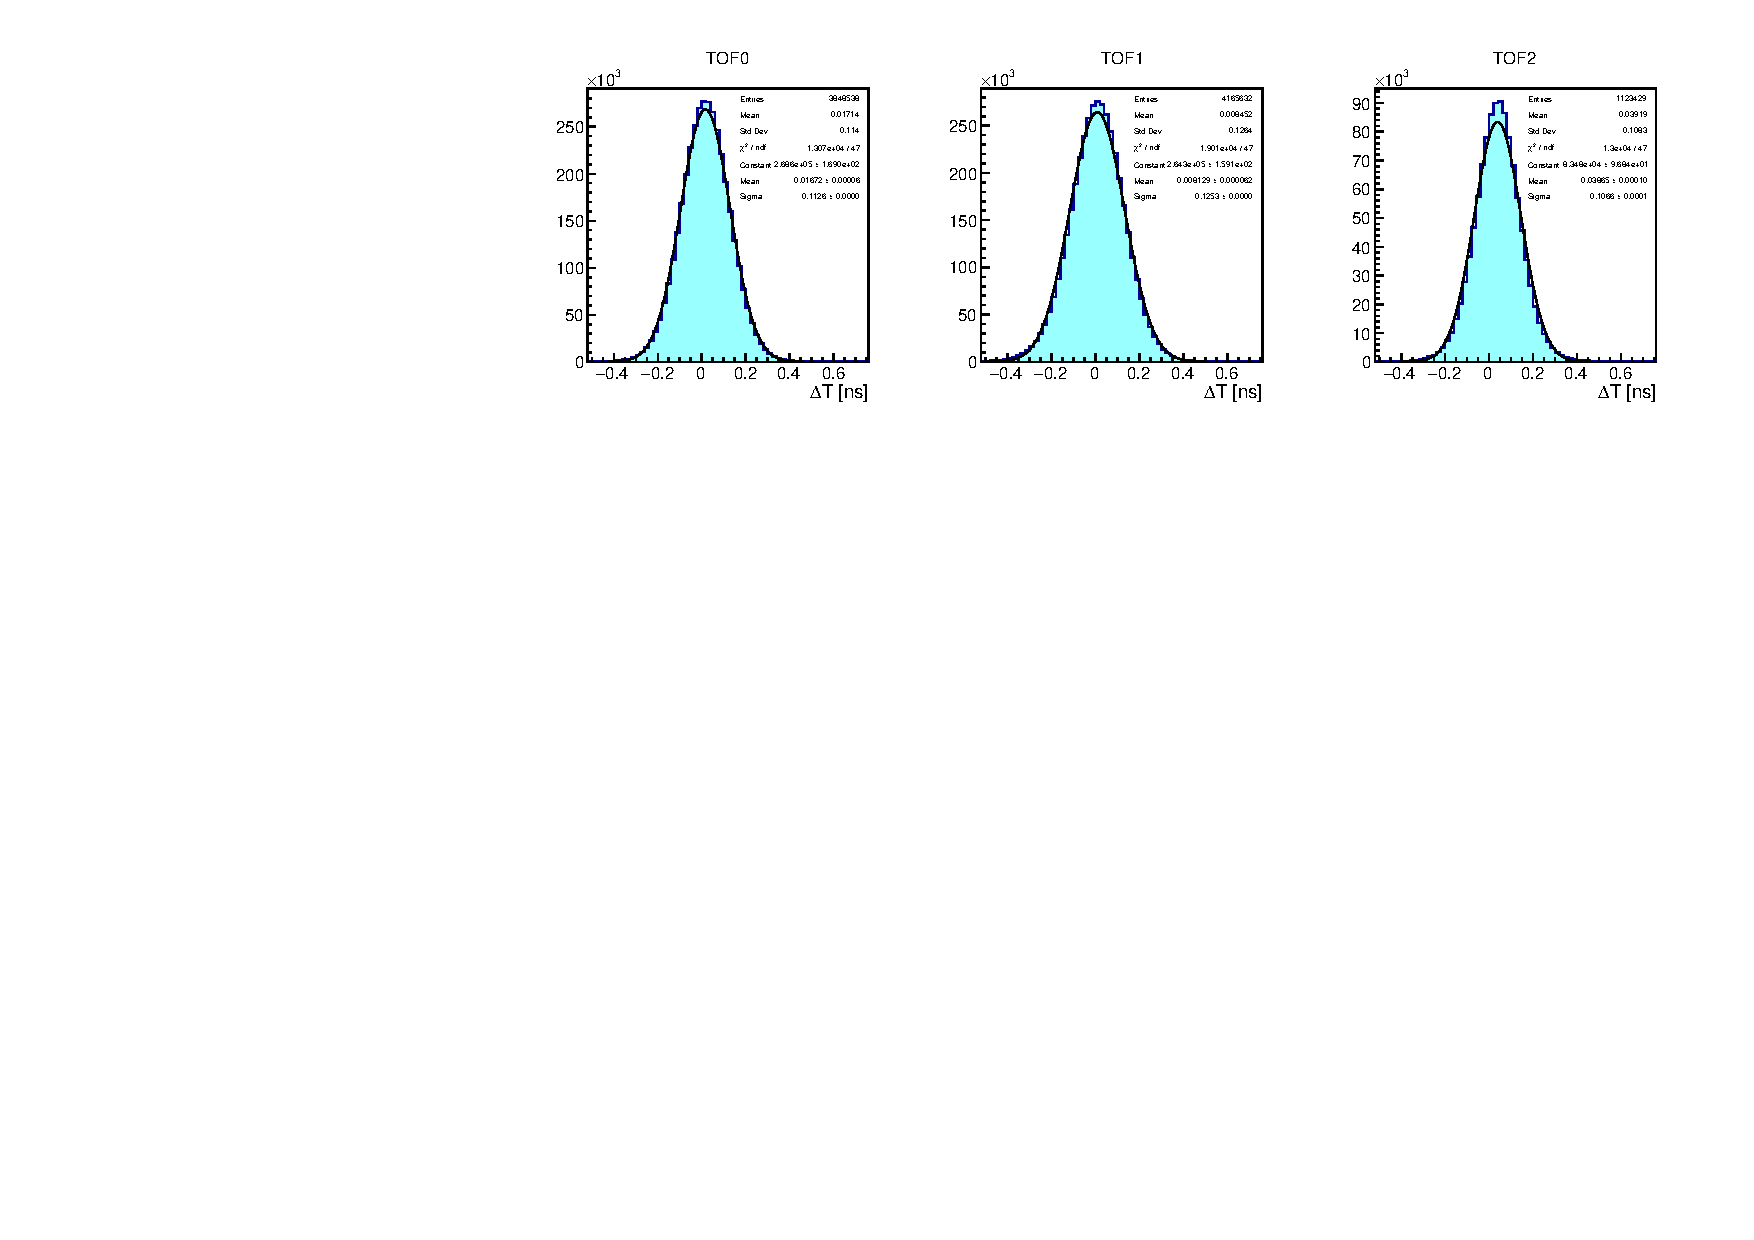
\includegraphics[width=15cm]{07_overall_slab_dt} \\
  \caption{}
  \label{fig:SlabDtAll}
  \end{center}
\end{figure}


\begin{figure}
  \begin{center}
  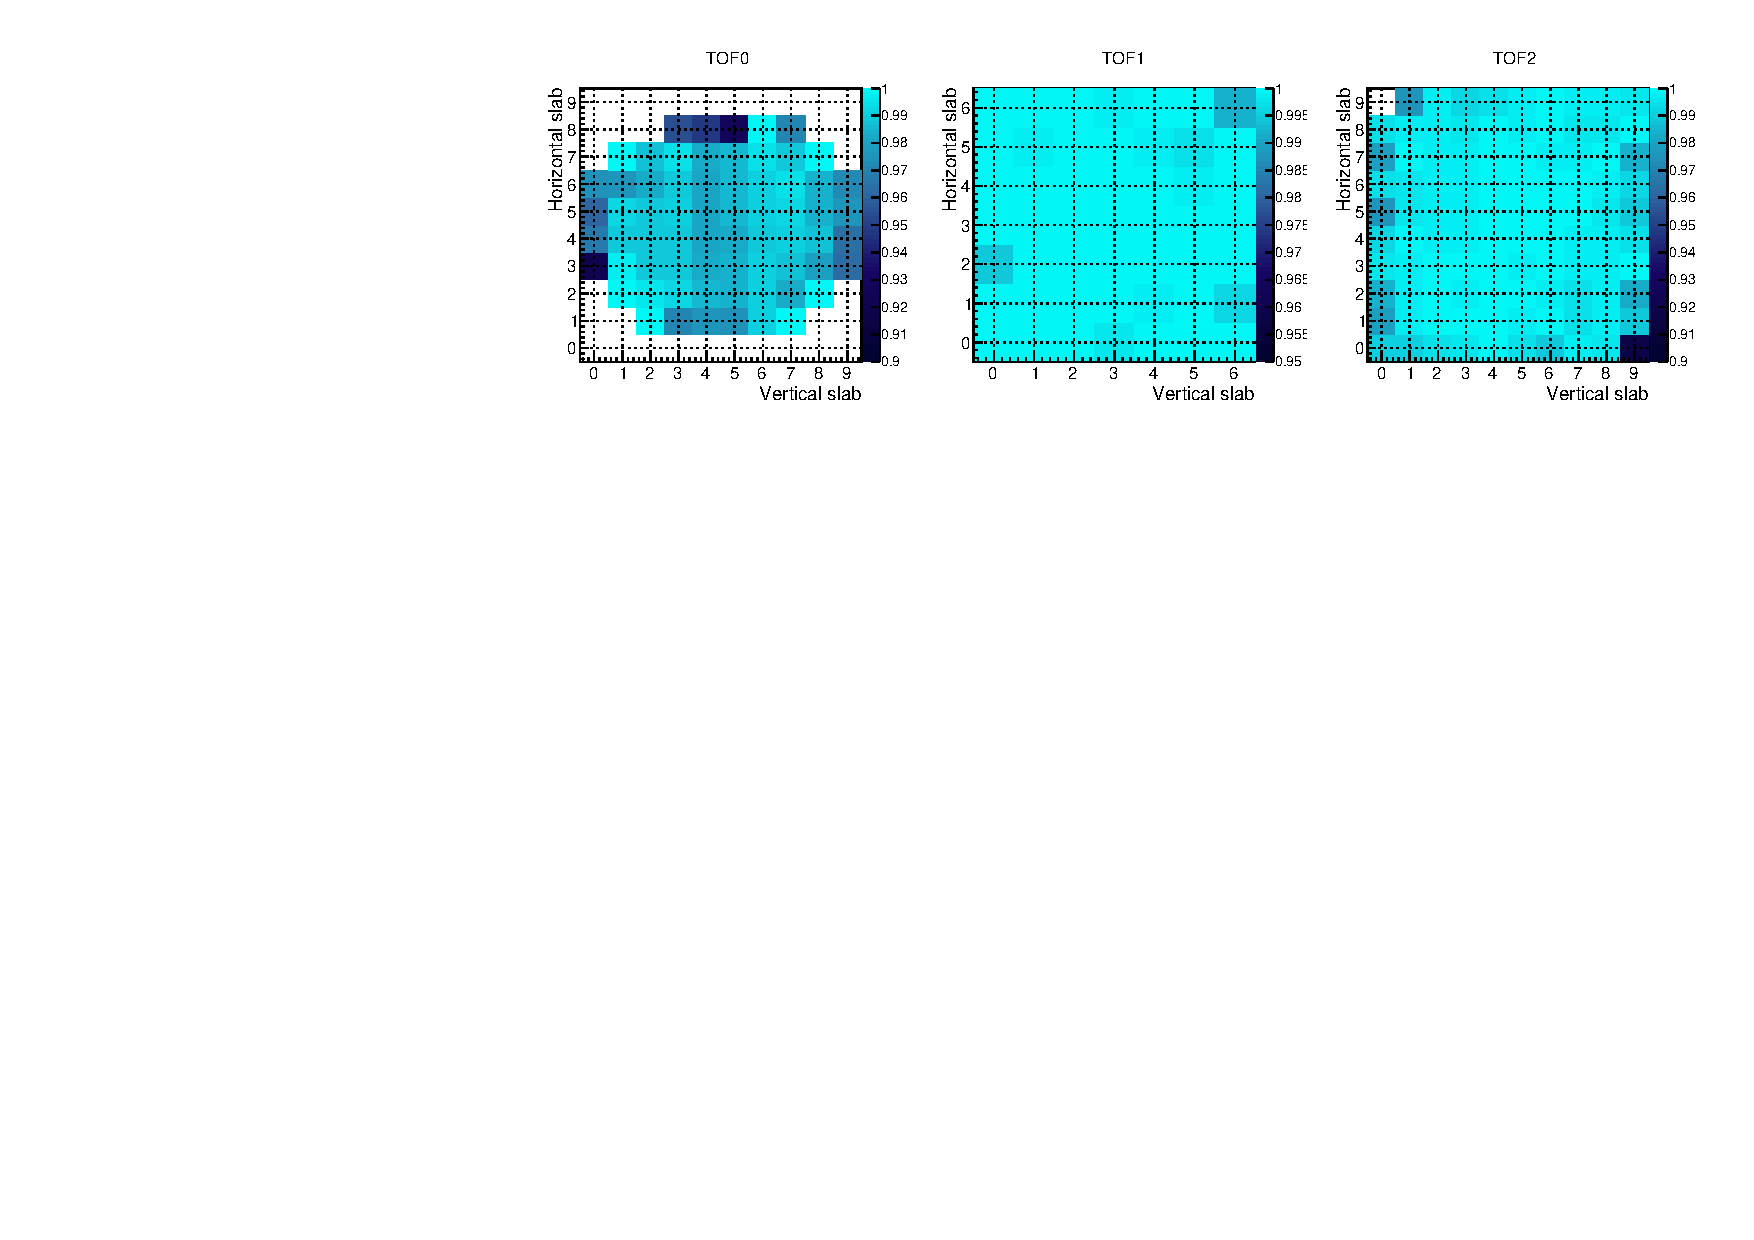
\includegraphics[width=15cm]{08_sp_eff_by_pixel_2d} \\
  \caption{}
  \label{fig:SpEffByPixel}
  \end{center}
\end{figure}




\subsection{Calibration Method}

Describe the method. Based on MICE note 251.

\malert{TOF NIMA paper says that measured time resolution of the CAEN
  TDC was 22~ps/count, as opposed to declared 25~ps!}

Some description of the calibration method is also described in the paper.



\subsubsection{Time Walk Correction}

\malert{Fig of a selected PMT TW 2D hist. + Profile + Fit}
\malert{Fig of residual TW.}
\malert{Fig of Slab DT before TW correction and after.}

Time walk was considered to be constant property of each channel. The
same correction was used for all runs.


\subsubsection{Trigger Delay Correction}


\subsubsection{T0 Correction}





\subsection{Reconstruction}


\subsection{Performance}
\label{SubSect:TOF_Performance}

\malert{Several figures are already in the TOF NIMA paper.}

{\color{red}
Figures to show up here:
\begin{itemize}
\item Slab DT - selected slabs/counters + overall TOFs
\item ToF10 - + detail of electron peak
\item Space-point reconstruction efficiency - shows that slab hits are
  within the required cut, inefficiency from only single slabs hit by
  different particles in the given spill/bunch
\item particle detection efficiency - how to show?
\end{itemize}
}

\subsubsection{Low-level Characterisation}
{\color{red}
  \begin{itemize}
  \item PMT charge correlation PMT0 vs PMT1 - maybe, if relevant
  \item Residual TW - this should go to the calibration section
  \item Slab DT
  \end{itemize}
}

\subsubsection{Time-of-Flight Resolution and Efficiency}
{\color{red}
  \begin{itemize}
  \item Resolution
    \begin{itemize}
    \item Slab DT for all TOFs, show similar performance, although
      they have different construction.
    \end{itemize}
  \item Efficiency
  \end{itemize}
}

%%% Local Variables:
%%% mode: latex
%%% TeX-master: "../Systems-performance"
%%% End:
